%! TeX program = xelatex
\documentclass[fontset=none]{ctexart}
\input{../note-setup.tex}

\title{Capacitated Two-Echelon Location Routing Problem with Drone-Truck Synchronization}
\author{Chen Huaneng}
\date{\today}
\setauthoremail{huanengchen@foxmail.com} % 笔记作者的邮箱

\begin{document}

\maketitle

\section{文献综述}

近年来，电子商务与同城配送需求急剧增长，城市物流网络面临巨大效率压力。两级物流系统通过引入卫星仓库（如前置仓、配送中心等），将运输过程拆分为“干线运输”和“支线配送”，能够显著降低配送成本并提高服务响应速度\cite{martinez-salazarSolvingBiobjectiveTransportation2014,prodhonSurveyRecentResearch2014,chaoOptimizationTwostageLocation2019}。同时，无人机技术的成熟使得车辆与无人机协同配送的模式受到广泛关注\cite{murrayFlyingSidekickTraveling2015,zhouMultitripUAVUGVDelivery2025}。本节先回顾与本研究最相关的两级选址-路径问题（Two-Echelon Location Routing Problem，2E-LRP），然后介绍选址-路径问题（Location Routing Problem，LRP）和车辆与无人机协同配送（Vehicle Routing Problem with Drone，VRP-D）相关的研究文献，并分析先前文献中存在的空白，为后续模型构建奠定基础。

\subsection{两级选址-路径问题研究现状}
两级选址-路径问题（Two-Echelon Location Routing
Problem，2E-LRP） 是标准 LRP 向多级物流网络的重要扩展，近年来受到越来越多研究者的关注，\cref{fig:2E-LRP}展示了 2E-LRP 配送网络的拓扑结构与运作流程。根据 Cuda 等人的系统综述\cite{cudaSurveyTwoechelonRouting2015}，2E-LRP 是一个包含了三个不相交顶点集合（潜在仓库、潜在卫星、顾客）的两级配送网络：第一级为仓库到卫星（或卫星之间）的干线运输，第二级为卫星到顾客（或顾客之间）的支线配送。与标准 LRP 相比，2E-LRP 需要同时决策卫星和仓库的选址、两级车辆的路径以及货物在卫星处的中转流量，且货物必须强制经过卫星仓库中转，且卫星和仓库的建设都需要相应的成本。

\begin{figure}[!htb]
    \centering
    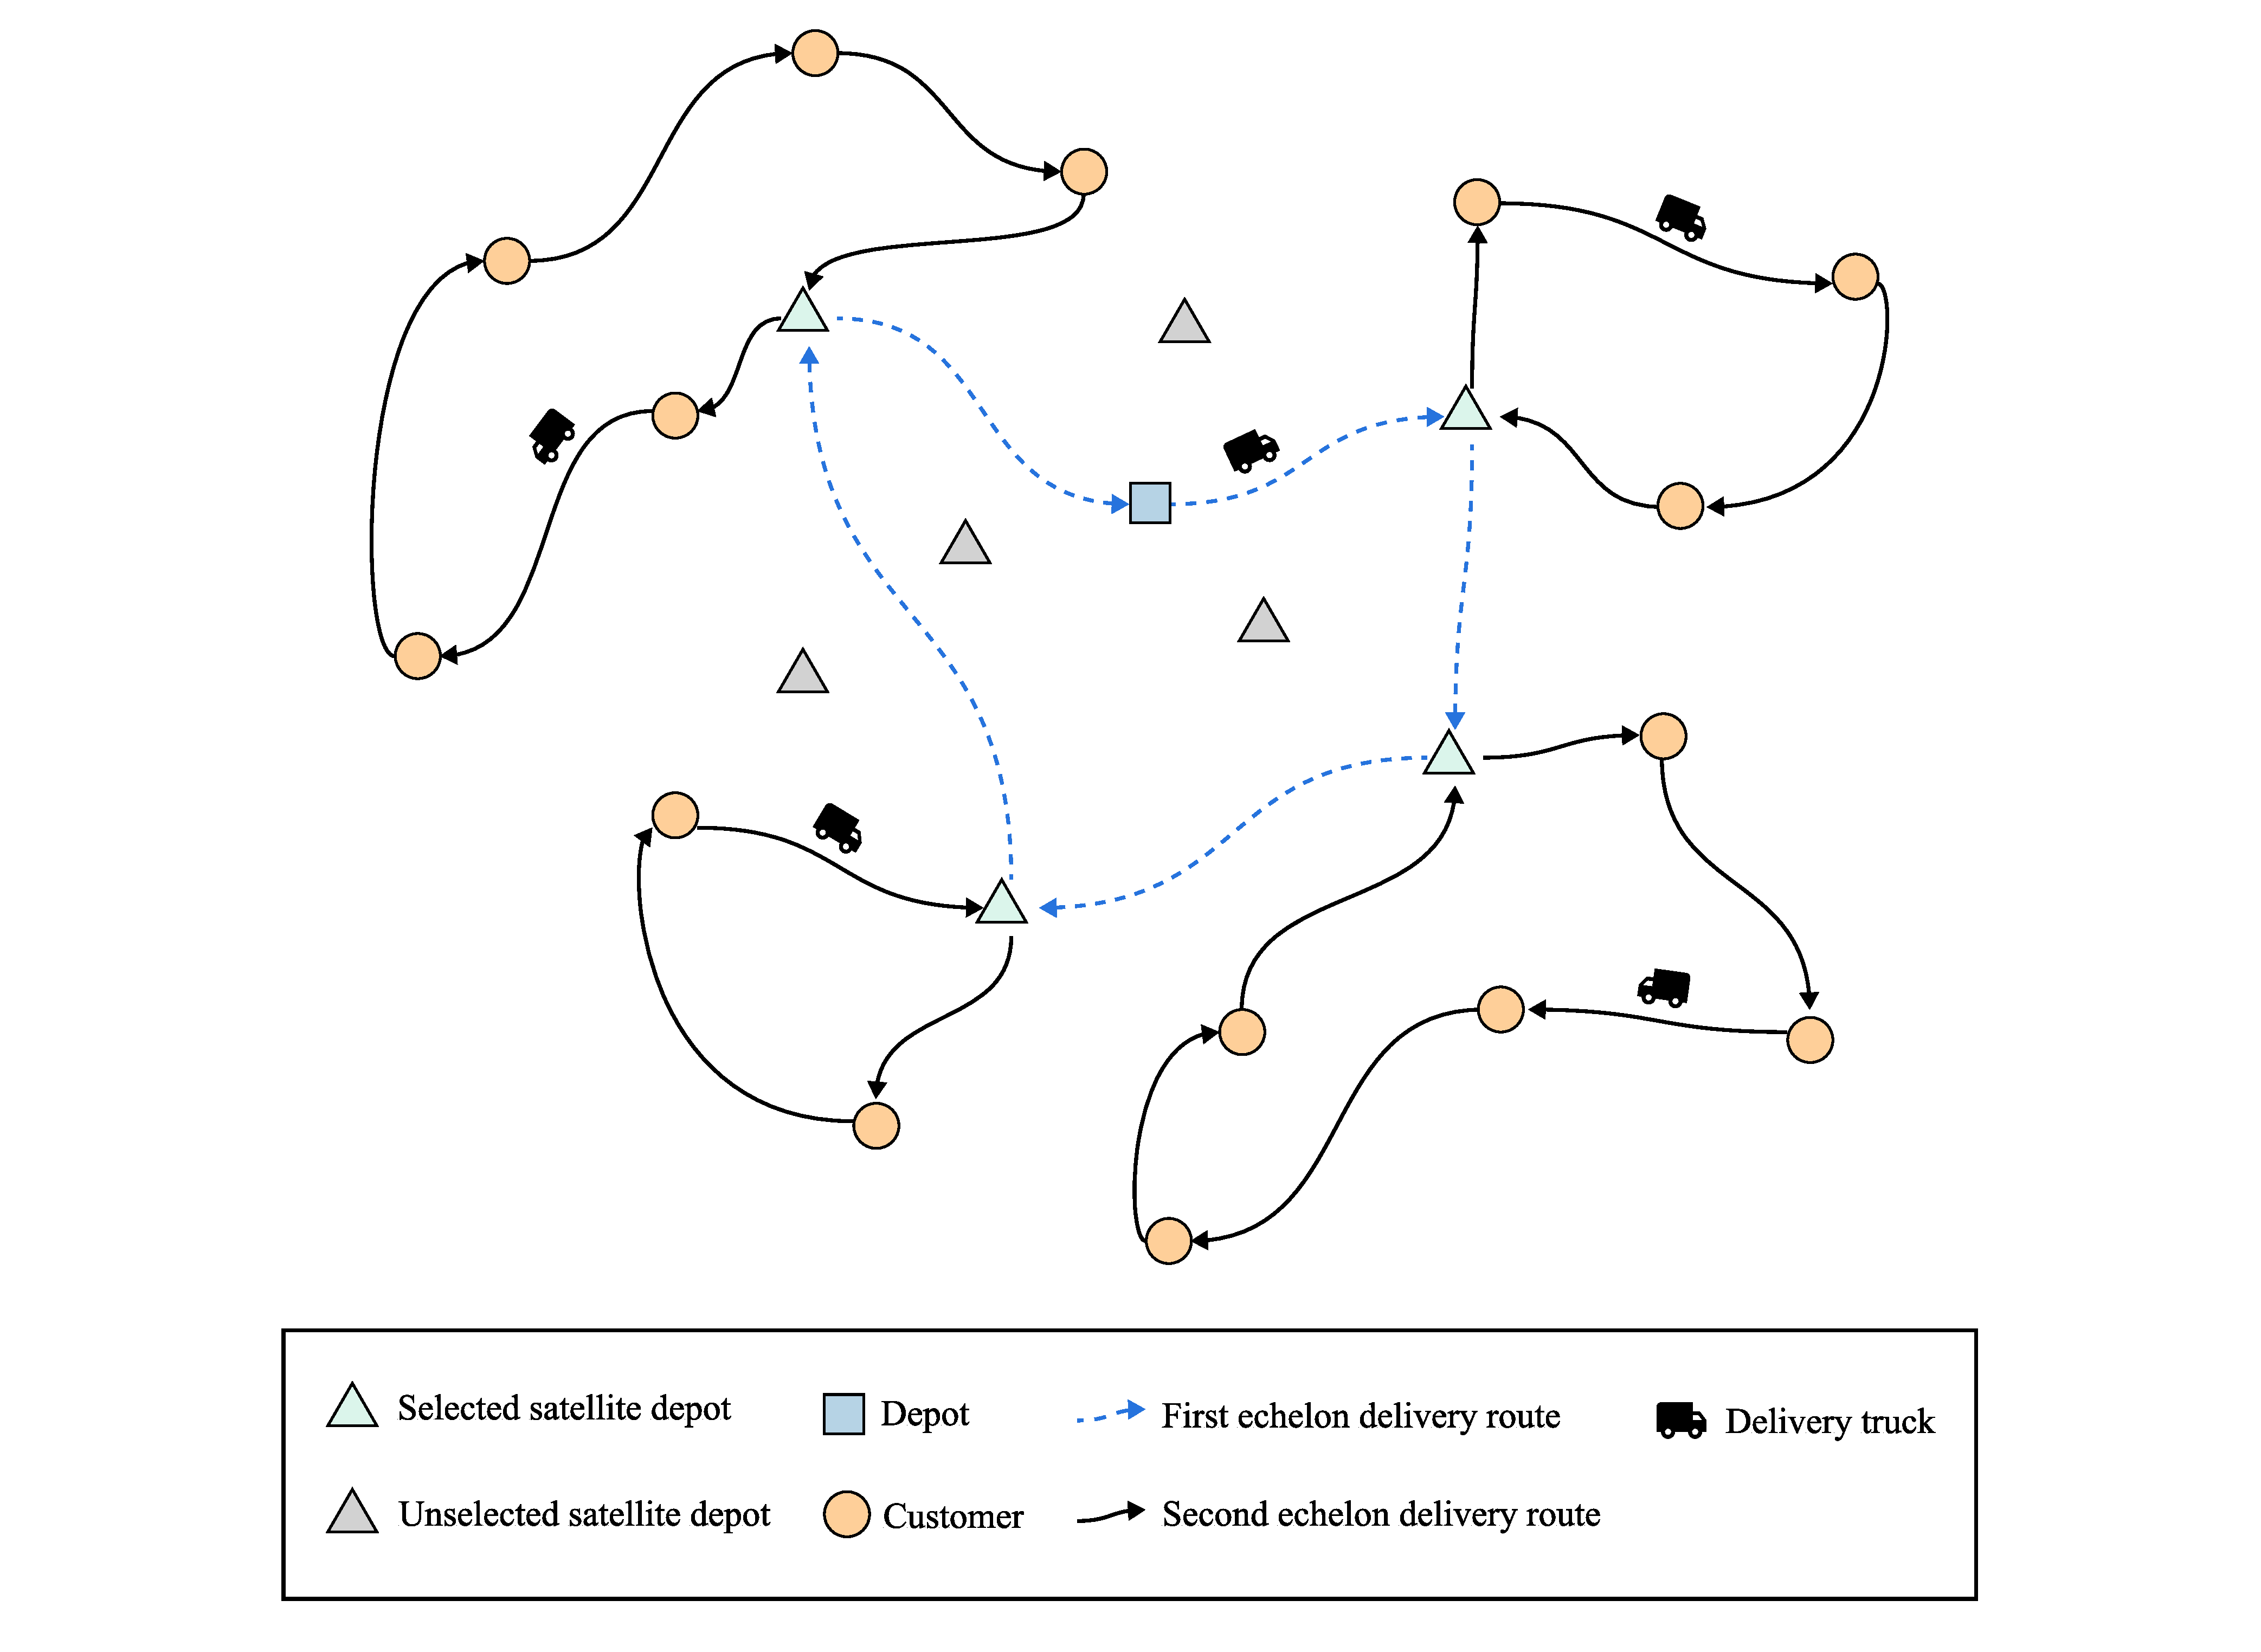
\includegraphics[width=0.8\linewidth]{image/2E-LRP.pdf}\\
    \caption{两级选址-路径问题配送网络示意图}\label{fig:2E-LRP}
\end{figure}

早期的2E-LRP研究多集中在考虑第二阶段的卫星仓库的选址决策上\cite{nguyenSolvingTwoechelonLocation2012, nguyenMultistartIteratedLocal2012}，在后续与2E-LRP相关的研究中最基础也研究最多的问题是有容量限制的两级选址-路径问题（Capacitated 2E-LRP，2E-CLRP）\cite{cudaSurveyTwoechelonRouting2015}，本研究也属于2E-CLRP的一个变体。在2E-CLRP中，第一层级只有一个仓库，并且第一级和第二级的车辆和仓库均有容量限制，同一层级的车辆是同质的，即车辆速度和容量限制等均相同\cite{aliIntegratedSequentialAlgorithms2025}。将选址和路径规划决策集成到一个双层方案中的想法可以追溯到Jacobsen和Madsen\cite{jacobsenComparativeStudyHeuristics1980}以及Madsen的研究工作\cite{madsenMethodsSolvingCombined1983}。但是，2E-CLRP最早是由Boccia等人进行了形式化描述\cite{bocciaMetaheuristicTwoEchelon2010}，作者介绍了该问题并基于Tuzun和Burke在解决LRP中使用的两阶段迭代方法（two-phase iterative approach）\cite{tuzunTwophaseTabuSearch1999}，提出了一种基于禁忌搜索（Tabu Search）的启发式方法，该算法主要将问题切分为两个阶段，首先确定设施的数量和位置，然后进行路径规划，并且采用先构建第二阶段的路径再构建第一阶段路径的自底向上的方案，并对包含最多5个仓库、20个卫星仓库和200个顾客节点的实例进行了计算实验。此外，Boccia等人还提出了三种混合整数规划公式，其中基于车辆索引变量（vehicle index variables）的公式表现优于双索引弧变量（two-index arc variables）公式，由此确立了大部分后续文献中采用车辆索引变量建模的传统\cite{sennaTwoechelonLocationroutingProblem2026}。

然而，Senna等人对这一传统提出了挑战\cite{sennaTwoechelonLocationroutingProblem2026}，作者对2E-LRP的紧凑公式进行了系统的比较分析，提出了两种基于双索引弧变量的新型紧凑公式：一种采用二元分配变量确保车辆返回其出发设施，另一种则采用连续分配变量追踪目的节点的出发设施，从而避免了二元分配变量的使用。作者还用商品流（commodity flow-based）约束改进了Boccia等人\cite{bocciaMetaheuristicTwoEchelon2010}基于车辆索引变量的公式。理论分析表明，两种新型双索引公式的线性规划松弛均严格强于车辆索引公式。大规模计算实验在Gurobi上对源自5个经典基准集（其中两个数据集来自Nguyen等人\cite{nguyenSolvingTwoechelonLocation2012}，另外三个数据集来自Contardo等人\cite{contardoLowerUpperBounds2012}）并剔除超大规模（200个顾客）后的131个基准算例的评估显示：基于车辆索引变量的传统公式在仅含50个顾客的算例上即无法找到可行解，而基于连续分配变量的双索引公式是唯一能在所有算例上找到可行解的公式，最优解个数接近传统公式的三倍，平均运行时间降低31.43\%，平均下界提高18\%。结合所提有效不等式，该研究在上述131个算例的测试中取得了突破性进展：一方面，成功提升了125个算例的历史最佳已知下界；另一方面，首次为55个算例严格证明了全局最优性。这些成果充分证明了双索引弧变量公式在2E-LRP中显著优于长期被文献视为标准的车辆索引变量公式。

Contardo等人则提出了一种双索引车辆流模型（two-index vehicle flow formulation）\cite{contardoLowerUpperBounds2012}，该模型是能够对小规模和中等规模实例求得最优解的分支切割算法（Branch and Cut，B\&C）的基础，该方法主要通过对Belenguer等人\cite{belenguerBranchandCutMethodCapacitated2011}和Contardo等人\cite{contardoComputationalComparisonFlow2013}关于CLRP（Capacitated Location Routing Problem）的论文中推导出的多种有效不等式进行加强，作者还引入了自适应大邻域搜索算法（Adaptive Large Neighborhood Search，ALNS）作为启发式算法，该算法在解决2E-CLRP问题中较其他启发式算法更优。而Ali等人则首次针对需求不确定条件下的鲁棒2E-CLRP（robust 2E-CLRP）展开研究\cite{aliIntegratedSequentialAlgorithms2025}，假设第二层级顾客的需求为随机变量，通过鲁棒优化方法构建鲁棒对偶模型，使得规划的路径在不确定性集合内所有需求实现下均保持可行。在求解算法上，作者设计了集成方法（包括ALNS启发式和分支切割精确算法）以及四种序列分解方法，计算实验表明，集成方法在解质量上显著优于序列方法，早期集成位置与路径决策对于降低两级配送网络总成本至关重要。在精确算法方面，Contardo等人则进一步发展了分支切割方法（B\&C）\cite{contardoExactAlgorithmBased2014}，Tian和Hu则提出了分支定价算法（Branch and Price，B\&P）\cite{tianBranchandpriceMethodTwoechelon2023}，为2E-CLRP的精确求解提供了新的途径。

近年来，少数学者开始尝试将车辆-无人机协同配送引入两级选址-路径框架中，以应对突发公共卫生事件或冷链生鲜品配送等特殊场景。Zhang和Li针对疫情背景下的易腐品配送问题，提出了一个包含“无接触式”配送站点选址与车辆-无人机协同路径的联合优化模型，目标是最小化总成本与易腐品产品价值损失，并设计了改进的K-means聚类（K-means clustering）与扩展的非支配排序遗传算法（extended Non-dominated Sorting Genetic Algorithm-II，NSGA-II）相结合的两阶段混合启发式算法\cite{zhangCollaborativeVehicledroneDistribution2023}。该研究通过成都市的案例验证了协同配送模式相比纯车辆配送可节省约34.75\%的总成本，并显著降低易腐品的价值损失。Li和Zhang则进一步将问题拓展至冷链运输场景\cite{liMultiechelonLocationRouting2026}，首次同时考虑两类设施选址（中转站与无人机起降点）、多级路径规划以及病毒传播风险，提出了多目标混合整数规划模型与基于分解的混合元启发式算法（hybrid multi-objective metaheuristic approach）。该研究在重庆市的实际案例中表明，合理的双层级站点布局与车辆-无人机协同可有效降低经济成本、配送时间与感染风险。Meng等人针对城市复杂路网中的血液配送问题\cite{mengLocationroutingOptimizationUAV2024}，提出了车辆-无人机协同的选址-路径优化模型，同时决策配送站和血液中心的选址以及车辆-无人机协同的路径规划。该研究考虑了血液的短保质期和异质性特点，建立中间站点作为二级配送站点，并采用改进的K-means聚类算法和自适应遗传算法（adaptive genetic algorithm）的两阶段混合启发式算法进行求解。基于上海市真实路网数据的案例研究表明，相比传统纯车辆配送模式，车辆-无人机协同模式可降低12.65\%的总成本并缩短37.5\%的整体配送时间。敏感性分析进一步探讨了无人机数量、车辆数量和司机工资等因素对系统性能的影响。Zhou等人提出了带释放时间约束的多行程无人机-无人车两级配送网络设计问题\cite{zhouMultitripUAVUGVDelivery2025}，联合优化对接枢纽选址、两级车队规模及多行程路径调度，每个包裹具有独立释放时间和交付截止时间，两级车辆均允许在规划周期内执行多次行程。作者建立了混合整数线性规划模型，并设计了基于自适应大邻域搜索的定制启发式算法，香港九龙区的实际案例表明该算法在大规模实例中能够在合理时间内产生高质量解。然而，该研究仅考虑单层级枢纽选址，第二级配送完全由地面无人车承担。Dukkani提出了一类考虑不确定性的卡车-无人机协同配送选址-路径问题\cite{dukkanciTruckDroneDelivery2026}，该问题联合优化停车场选址、卡车行驶路径及商店到停车场和无人机的分配，卡车在停车场作为移动起降平台，无人机从停车场起飞向末端取件点执行配送。模型同时考虑需求不确定性和无人机飞行时间不确定性，采用两阶段随机规划建模，并设计了场景分解精确算法及多种改进策略。基于伊斯坦布尔真实数据集的实验表明，所提算法可在所有实例中求得最优解，且随机解相较于确定性解在部分实例中可带来最高约6.56\%的目标值改善。但该研究仅考虑无人机的配送，未涉及无人机和卡车协同服务顾客并在协同过程中卡车单独配送的优化。

已有文献大多将二级配送限定为纯车辆运输或者只考虑车辆和无人机分别配送，极少考虑无人机和车辆的协同配送，这为本文的研究提供了切入点。

\subsection{选址-路径问题研究现状}
选址-路径问题（Location Routing Problem，LRP）结合了物流中的两个基本的规划任务，即设施的选址决策和车辆路径的决策。将这两种规划任务彼此独立地进行决策，可能会导致整体目标非最优\cite{salhiEffectIgnoringRoutes1989, drexlSurveyVariantsExtensions2015}，即使选址是基于长期规划而做出的决策也仍然可能导致整体目标非最优\cite{salhiClusterInsertionHeuristic1999}。因此，如何有效地同时优化选址和路径规划成为了物流学界研究的热门课题\cite{albareda-sambolaLocationRoutingLocationArcRouting2015, balakrishnanIntegratedFacilityLocation1987, drexlSurveyVariantsExtensions2015, lopesTaxonomicalAnalysisCurrent2013, marinakisLocationRoutingProblem2008, nagyLocationroutingIssuesModels2007, prodhonSurveyRecentResearch2014, schneiderSurveyStandardLocationrouting2017, cavagniniRecentDevelopmentsLocationrouting2026, marinakisLocationRoutingProblem2024, wandeltLiteratureReviewHub2025, schifferVehicleRoutingLocation2019a}。

标准的路径-选址问题如果只有一个潜在可以选择的设施且车辆队列仅包含一辆无限容量的卡车，则退化为旅行商问题（Traveling Salesman Problem，TSP），已知TSP是NP-Hard\cite{computers-and-intractability}，因此标准的以及拓展的路径-选址问题也是NP-Hard。在路径-选址问题（LRP）中，必须做出至少以下两种相互依赖的决策类型：

\begin{enumerate}[label = (\roman*)]
    \item 从有限或者无限的潜在设施集合（如工厂、仓库、配送中心、枢纽等）中选择哪些设施启用。
    \item 使用给定的车辆，应建立哪些车辆路径来服务给定的需求点。
\end{enumerate}

并且在 LRP 中，路径的选择不能隐含选址的决策，即选址的决策和路径的决策不能够相互依赖，Schneider和Drexl指出，当满足以下三个条件之一时路径决策和选址决策是相互独立的\cite{schneiderSurveyStandardLocationrouting2017}：

\begin{enumerate}[label = (\roman*)]
    \item 启用设施存在固定成本或使用设施存在与体积相关的可变成本；
    \item 必须从某个更大的集合中选择恰好或最多一定数量的设施；
    \item 设施具有某种容量的限制。
\end{enumerate}

自Salhi和Rand\cite{salhiEffectIgnoringRoutes1989}以及Salhi和Nagy\cite{salhiClusterInsertionHeuristic1999}的开创性工作之后，LRP的研究在理论和应用层面均取得了长足发展。早期的综述（如Balakrishnan等人\cite{balakrishnanIntegratedFacilityLocation1987}，Min等人\cite{minCombinedLocationroutingProblems1998}）奠定了问题基础，而Nagy和Salhi的综述则系统梳理了2006年前的模型与方法\cite{nagyLocationroutingIssuesModels2007}。在标准LRP的定义上，后续研究普遍遵循Schneider和Drexl所归纳的三个准则：启用设施存在固定成本、需从更大集合中选择有限数量设施、或设施存在容量限制\cite{schneiderSurveyStandardLocationrouting2017}。基于此，标准LRP通常被界定为确定性、静态、离散、单层级、单目标的问题，其中每个顾客必须被恰好访问一次，且不涉及库存决策\cite{drexlSurveyVariantsExtensions2015, cavagniniRecentDevelopmentsLocationrouting2026}。

在精确算法方面，早期研究致力于通过分支定价（Branch and Price）或分支切割（Branch and Cut）求解小规模实例。Berger等人利用分支定价法解决了含路径长度约束的LRP，作者通过Feillet等人提出的标签算法（labeling algorithm）求解生成新路径的子问题\cite{feilletExactAlgorithmElementary2004}，可在两个小时内求解含10个潜在设施以及50--100个顾客的算例\cite{bergerLocationRoutingProblemsDistance2007a}。Akca等人提出了结合有效不等式的分支定价算法，但求解能力仍局限在5个设施及40个顾客左右\cite{akcaBranchandPriceAlgorithmCombined2009}。Belenguer等人通过引入多种有效不等式，包括源自容量约束车辆路径问题（Capacitated Vehicle Routing Problem，CVRP）的切割，增强了分支切割算法，该算法优于Akca等人提出的分支定价算法\cite{akcaBranchandPriceAlgorithmCombined2009}，成功求解了含5个设施及50个顾客的算例\cite{belenguerBranchandCutMethodCapacitated2011}。Baldacci等人在Akca等人提出的模型基础上\cite{akcaBranchandPriceAlgorithmCombined2009}，提出了一种类似集合划分（set-partitioning-like）的新颖精确方法，通过动态规划与对偶上升法（dual ascent methods）等不同的界限分析技术生成紧的下界，并将原LRP分解为有限个带容量限制的多仓库车辆路径问题（multi-capacitated depot vehicle routing problems），该方法显著提升了求解规模，能够求解含14个潜在仓库和199个顾客的实例\cite{baldacciExactMethodCapacitated2011}。Contardo等人在此基础上进一步发展了弧变量和路径变量两种建模框架，并提出了多种新的有效不等式，实验的计算结果表明，提出的方法不仅能够求解Baldacci等人公开的所有实例\cite{baldacciExactMethodCapacitated2011}，还首次解决了四个此前未决的算例，并改进了三个算例的最优上界\cite{contardoComputationalComparisonFlow2013, contardoExactAlgorithmBased2014}。然而，精确算法仍然难以在有效时间内求解更大规模的算例，直到Liguori等人提出的分支-切割-定价（branch-cut-and-price）算法，通过引入非鲁棒的路由装载背包割（nonrobust route load knapsack cuts），才首次能够稳定求解含300个顾客和20个候选设施的较大规模算例，标志着标准LRP精确求解能力的重要突破\cite{liguoriNonrobustStrongKnapsack2023}。

鉴于LRP的NP-Hard特性，启发式与元启发式算法一直是研究主流。早期方法多采用两阶段分解策略：先确定设施选址与顾客分配，再为每个启用的设施规划车辆路径。Prins等人提出的贪婪随机自适应搜索过程（Greedy Randomized Adaptive Search Procedure，GRASP）结合路径重连（path relinking），通过随机化的扩展Clarke-Wright算法（Randomized Extended Clarke and Wright Algorithm，RECWA）构造初始解，并设计多样化和强化阶段来搜索设施配置空间\cite{nguyenSolvingTwoechelonLocation2012}。后来Prins等人又进一步提出了带种群管理的模因算法（Memetic Algorithm with Population Management，MA|PM）\cite{prinsMemeticAlgorithmPopulation2006}，通过采用车辆巨型路线编码和动态规划分割技术，实现了相比于后来Prins等人提出的算法的解质量提升，但需要花费更多的求解时间\cite{prinsSolvingCapacitatedLocationRouting2007}。这些工作在经典的Tuzun和Barreto\cite{tuzunTwophaseTabuSearch1999}，Prins等人\cite{nguyenSolvingTwoechelonLocation2012, prinsSolvingCapacitatedLocationRouting2007}和Barreto等人\cite{barretoUsingClusteringAnalysis2007}的算例集上取得了当时的最优结果。

随后的十年间，启发式算法在搜索机制和问题扩展上持续创新。Yu等人设计了高效的模拟退火（Simulated Annealing，SA）算法，改进了多个已知最优解\cite{yuSimulatedAnnealingHeuristic2010}。Duhamel等人将GRASP与进化局部搜索（Evolutionary Local Search，ELS）结合，进一步提升了求解质量\cite{duhamelGRASPxELSApproachCapacitated2010}。Hemmelmayr等人提出的自适应大邻域搜索（Adaptive Large Neighborhood Search，ALNS）不仅高效求解两级车辆路径问题（Two-Echelon Vehicle Routing Problem，2E-VRP），还能通过转换求解标准LRP，展现了方法的通用性\cite{hemmelmayrAdaptiveLargeNeighborhood2012}。Escobar等人提出了融合变邻域搜索（Variable Neighborhood Search，VNS）和粒度禁忌搜索（Granular Tabu Search，GTS）的混合算法，在计算效率与解质量之间取得了良好平衡\cite{escobarGranularVariableTabu2014, escobarTwophaseHybridHeuristic2013}。Ting和Chen则探索了多蚁群协同优化（multiple ant colony optimization）框架，三个蚁群分别处理选址、分配和路径决策三个任务\cite{tingMultipleAntColony2013}。Schneider和Löffler提出了一种基于树搜索的算法（Tree-Based Search Algorithm，TBSA），系统性地探索设施配置空间，并采用包含14种算子的复合大邻域进行路径优化，该算法在处理含600个顾客和30个设施的大规模算例时表现出优异的扩展性和鲁棒性，并在经典的算例集中发现了多个新的最优解结构\cite{schneiderLargeCompositeNeighborhoods2019}。此外，部分研究致力于发展近似算法，例如Heine等人提出了基于最小生成树和聚类问题的多项式时间近似算法，虽然不能够直接获得最优解，但能处理超大规模实例，为实际应用提供了保障\cite{carrascoheineBifactorApproximationLocation2023}。

尽管标准LRP的研究已相对成熟，但为应对现实物流系统的复杂性，研究焦点逐渐向更具挑战性的变体扩展。其中，多级物流网络（特别是两级LRP） 被认为是近十年来最重要的模型扩展之一\cite{drexlSurveyVariantsExtensions2015}。两级LRP（Two-echelon Location Routing Problem，2E-LRP）将配送网络划分为干线运输（第一级）和支线配送（第二级），通过引入中转设施（如卫星仓库）实现成本聚合与高效分拨。多级物流网络（multi-echelon/N-echelon VRP/LRP）术语最早是由Perboli等人提出的，Perboli等人系统定义了两级容量约束车辆路径问题（Two-Echelon Vehicle Routing Problem，2E-VRP）并提出了基于弧变量的混合整数规划（Mixed Integer Programming，MIP）模型\cite{perboliTwoEchelonCapacitatedVehicle2011}。随后，Crainic等人\cite{crainicMultistartHeuristicsTwoEchelon2011}、Nguyen等人\cite{nguyenSolvingTwoechelonLocation2012, nguyenMultistartIteratedLocal2012}、Contardo等人\cite{contardoLowerUpperBounds2012}分别提出了多起点启发式（multi-start heuristic）、GRASP、ALNS和精确算法（Branch and Cut algorithm）。这些研究一致表明，在恰当的设施布局下，两级系统相较于单级系统能显著降低总配送成本，尤其在城市物流场景中具有巨大潜力。然而，现有研究多忽略了第二级物流网络通过无人机协同来进行配送优化，这为后续研究提供了切入点。

综上所述，选址-路径问题经过数十年的发展，已在问题定义、模型构建和算法设计方面形成了较为完整的体系。然而，随着电子商务、即时配送和城市物流的快速发展，传统的单级、纯车辆配送模式正面临挑战。一方面，两级或更多级物流网络的实践应用日益广泛，对其中转设施（卫星仓库、配送中心、前置仓等）的选址与路径联合优化提出了更高要求；另一方面，车辆与无人机协同配送作为一种新兴模式，能够利用无人机的空中直线路径和卡车的续航载重优势，进一步提升“最后一公里”的配送效率。将这两类扩展（多级网络与新型运载工具）进行整合，研究面向两级配送网络的卫星仓库选址与车辆-无人机协同路径问题，既是LRP领域自然的研究延伸，也具有显著的实际应用价值。

\subsection{车辆与无人机协同配送研究现状}
% INFO: 论文（DOI：10.1080/24725854.2022.2060535）和本文的模型很类似

车辆与无人机协同配送问题（Vehicle Routing Problem with Drone，VRP-D）是近年来物流优化领域的研究热点。该问题将传统卡车的长距离、大载重优势与无人机的高机动性、直线飞行能力相结合，旨在提升“最后一公里”配送的效率与灵活性。Murray和Chu首次提出利用车辆和无人机协同配送进行“最后一公里”配送\cite{murrayFlyingSidekickTraveling2015}，提出了TSP的两种变体，分别称为飞行助手旅行商问题（Flying Sidekick Traveling Salesman Problem，FSTSP）和并行无人机调度旅行商问题（Parallel Drone Scheduling Traveling Salesman Proble，PDSTSP）。在FSTSP中，一辆卡车搭载一架无人机进行配送任务，并且无人机每次飞行只能服务单个顾客点。该论文明确给出了基于弧的混合整数线性规划（Mixed Integer Linear Programming，MILP）模型，并且通过设计基于成本节约的大邻域搜索算法，对10--20个节点的实例进行了数值计算。这一工作为后来的车辆与无人机协同配送问题研究奠定了基础，其他学者在FSTSP基础上进行了大量的延伸拓展研究。

在FSTSP模型基础上，Ha等人首次以最小化服务成本为目标函数\cite{haMincostTravelingSalesman2018}，考虑了无人机和卡车因为等待另一方的时间成本，用改进的简单启发式算法和贪婪随机自适应搜索过程（Greedy Randomized Adaptive Search Procedure，GRASP）求解，并比较了最小服务时间和最小服务成本两种目标的解决方案异同。Agatz等人在之前的研究基础上基于最小化服务成本的目标函数建立了能够解决最多12个顾客点的最优整数规划（Integer Programming，IP）模型\cite{agatzOptimizationApproachesTraveling2018}，并提出了一种基于局部搜索和动态规划的启发式算法，通过对比最优结果和启发式算法的结果，验证了协同配送相较于纯卡车配送的优越性。Bouman等人同样以最小化服务成本为目标函数\cite{boumanDynamicProgrammingApproaches2018}，将精确求解方法用于更大规模的算例求解中，并通过基于Bellman-Held-Karp的三阶段动态规划方法进行求解，同时通过限制卡车和无人机分离时卡车可以访问的节点来加速运算。

Phan等人则将模型拓展到结合单辆卡车和多架无人机协同的包裹配送问题\cite{tuTravelingSalesmanProblem2018}，并称之为TSP-mD（Traveling Salesman Problem with multiple Drones），作者在论文中提出了一种基于自适应大邻域搜索（Adaptive Large Neighborhood Search，ALNS）的启发式算法来解决这一问题，并与GRASP进行了比较，证明了ALNS算法在效率上优于GRASP。Murray等人在FSTSP的基础上提出多无人机的混合整数线性规划数学模型\cite{murrayMultipleFlyingSidekicks2020}，并通过三阶段的启发式方法求解，并分析了五种不同的无人机耐力模型，发现使用过于简化的耐力模型可能会导致无人机无法安全返回。Poikonen等人同样对一辆卡车与多架无人机协同配送包裹的问题进行研究\cite{poikonenMultivisitDroneRouting2020}，目标是最小化所有包裹送达顾客地点的总路线完成时间，该问题允许无人机携带多个不同重量的包裹，并考虑了无人机的能耗函数，该函数取决于包裹重量和飞行距离。该论文采用RTS（Route，Transform，Shortest Path）启发式方法进行求解，发现增加无人机数量可以减少总路线完成时间，但存在边际收益递减的现象。

Kitjacharoenchai等人首次提出了mTSPD（multiple Traveling Salesman Problem with Drones）\cite{kitjacharoenchaiMultipleTravelingSalesman2019}，即多卡车与多无人机的协同配送问题，目标是最小化包裹配送的完成时间，文章提出了一个混合整数规划模型和一种基于插入启发式（Adaptive Insertion Heuristic，ADI）的算法，以解决大规模问题。Rinaldi等人设计并实现了几种启发式方法来解决这一问题\cite{rinaldiDevelopmentHeuristicApproaches2023}，包括局部搜索算法、两种混合遗传算法（可行解变体和不可行解变体）以及一种自定义的贪心算法，结果表明，遗传算法在提高配送效率方面表现最佳，尤其是在大规模实例中。Cui等人在之前的研究上更进一步\cite{cuiDynamicCollaborativeTruckdrone2024}，以最大化预期收益为目标函数，考虑了顾客随时可能出现的需求（即需求的不确定性）和无人机可以不在顾客节点起飞降落的情形，并使用分散学习和集中调度（decentralized learning and centralized dispatching）的方法来提高强化学习的表现。

针对多卡车与多无人机的协同配送且考虑卡车容量的问题（Vehicle Routing Problem with Drones，VRPD），Wang等人的研究旨在通过配备无人机的卡车车队来优化包裹配送\cite{wangVehicleRoutingProblem2017}，目标是最小化总配送时间，作者通过理论分析，探讨了使用无人机相比传统卡车配送在最坏情况下的时间节省潜力，并给出了多个关键结论和定理。在此基础上，Poikonen等人拓展了研究的例子\cite{poikonenVehicleRoutingProblem2017}，主要是针对无人机的电池容量、无人机面临空中障碍物以及考虑无人机和卡车的使用成本的情况，进一步拓展了使用无人机带来的潜在收益。Schermer等人将VRPD形式化为一个混合整数线性规划模型\cite{schermerMatheuristicVehicleRouting2019}，并引入了一系列有效的不等式以提高求解器的性能，由于求解器在处理大规模实例时性能有限，作者提出了一种基于问题结构的启发式方法，该方法通过分解问题来有效利用VRPD的结构特性，并且通过对比不同规模实例的结果，作者发现无人机的使用可以显著减少完成时间，且这种减少在不同规模的实例中都是一致的。

根据前文所述文献，车辆与无人机协同配送的相关研究可以根据车辆数量、车载无人机数量和是否考虑车辆容量分成四类：TSPD、TSP-mD、mTSPD和VRPD。这四类问题的区别如\cref{tab:tspd1}所示。

\begin{table}[!htbp]
    \centering
    \caption{车辆与无人机协同配送问题分类}\label{tab:tspd1}
    \begin{tabular}{cccc}
        \toprule[1pt] % 表头线宽1镑（point, pt）
        问题类型 & 车辆数 $n$ & 车载无人机数 $m$ & 是否考虑卡车容量 \\
        \midrule[0.75pt] % 表中间线宽0.75镑（point, pt）
        TSP-D & 1 & 1 & 是 \\
        TSP-mD & 1 & $m > 1$ & 是 \\
        mTSPD & $n > 1$ & $m \geq 1$ & 否 \\
        VRP-D & $n > 1$ & $m \geq 1$ & 是 \\
        \bottomrule[1pt] % 表尾线宽1镑（point, pt）
    \end{tabular}
\end{table}

从上述文献梳理可以看出，现有VRP-D研究虽然在问题变体与求解方法上取得了长足进展，但绝大多数模型默认采用单级配送网络结构，即卡车从中央仓库出发，完成配送后返回同一仓库。这种结构在城市物流中面临两个现实瓶颈：一是长距离行驶导致卡车配送时效下降；二是中央仓库的固定成本较高，难以灵活应对分散化的末端需求。同时，将卫星仓库选址与车辆-无人机协同配送进行联合优化的研究仍相对匮乏\cite{zhangCollaborativeVehicledroneDistribution2023,liMultiechelonLocationRouting2026}，现有文献多将卫星仓库位置视为已知输入，或仅考虑纯车辆的两级配送，或考虑无人机和车辆分别进行配送。因此，面向两级物流网络，研究卫星仓库的选址决策与车辆-无人机协同路径的联合优化问题，既是2E-LRP与VRP-D交叉领域的重要理论延伸，也具备显著的实际应用价值。

\section{问题描述}

% 可以拓展的方向
% 1. 卡车行驶时间不确定性和顾客需求不确定性（stochastic）
% 2. 周期性的决策问题，即周期性决定选址及路径规划（periodic）
% 3. 选址可以是在连续空间选址也可以在固定的集合中选址（discrete vs continuous）
% 4. 多级网络可以考虑在两级以上的配送网络（multiple echelons）
% 5. 考虑多目标（multiple objective）
% 6. 考虑多个选址之间物流的运输，即物流中心之间的货物运输（hub location-routing problem）
% 7. 考虑无人机的最大续航里程受到其携带的包裹重量的影响

给定一个物流配送网络$G = (V, A)$，该网络为一个完全图，网络中的节点包含一个郊区仓库$0$和一个待选的卫星仓库集合$S$以及一个需要配送的顾客集合$N$，为了方便建模，对每个仓库设置一个相应的虚拟仓库，郊区仓库的虚拟仓库为$0'$，卫星仓库$s \in S$的虚拟仓库为$s' \in S'$，网络的弧集合为$A = \{(i,j)|i,j \in V, i \neq j\}$。

首先由大型卡车将需要配送的货物从郊区仓库$0$运输到一个选择建设的卫星仓库节点集合$\hat{S} \subseteq S$，每个建设的卫星仓库都配有一辆卡车和一架相应的无人机负责配送，且每个顾客最多只能被卡车或者无人机服务一次，由卡车和无人机从卫星仓库出发进行协同配送，无人机和卡车都可以进行货物的单独配送，无人机进行配送的过程中卡车可以进行下一个顾客点的配送，但是无人机的配送受到自身最大载重$Q^D$和最大电量$E$的限制，需要在载重的约束下，并且在自身电量耗尽前到达和卡车的会合节点，无人机可以在会合节点等待卡车配送完成后会合，也可以卡车在会合节点等待无人机配送完成后会合，同样，卡车也受到最大载重$Q^T$的限制，即携带的无人机和包裹总重量不能超过卡车的最大载重$Q^T$，且每辆卡车最多只能携带一架无人机进行协同配送，目标是最小化经济成本，包括卡车和无人机的运输成本，卫星仓库的固定建设成本。

为简化问题并构建可行的数学模型，做出以下合理假设：

首先是无人机的能力限制。因为无人机起飞和回收的时间相比于卡车和无人机配送的时间来说很短，因此模型中不考虑无人机的起飞和降落时间。无人机在每次飞行任务结束后通过更换电池从而达到最大电量，因此每次无人机起飞时都有最大电量$E$，且卡车携带的无人机电池足够多，不考虑无人机换电池的时间。

其次是顾客需求特性。任一顾客既可以由卡车配送，也可以由无人机配送，当顾客被无人机或卡车服务后，无人机和卡车都不能再次访问该顾客，无人机不能重复访问同一个顾客，即卡车不能在同一个顾客节点等待无人机，从而不会产生无人机飞行路径是个环的情况，每个顾客节点都有充足的空间供无人机起飞和降落，且无人机在会合点需要等待卡车时会降落在地面等待，因此不需要考虑无人机等待卡车的成本。可供建设的卫星仓库数量足够多以至于所有的顾客都能被服务到，且大型卡车的载重能够满足所有卫星仓库的需求。

再次是协同规则约束。无人机的起飞和降落地点仅限于仓库或顾客位置。无人机和卡车只能够在顾客节点会合，不能在行驶过程中进行会合，在实际应用中，由于无人机降落在行驶过程中的卡车需要卡车和无人机的速度相匹配，而这个匹配的过程十分困难\cite{buchmueller2016landing}，并且无人机降低速度匹配卡车会降低无人机的配送效率，因此这里假设无人机和卡车只能在顾客节点会合。当卡车和无人机在某一节点会合时，如果卡车先到达，需等待无人机，若无人机先到达，则无人机等待卡车，但是无人机的等待时间不能超过无人机剩下的续航时间。每个卡车组的无人机都只能依赖于该卡车组的卡车，即该无人机不能在其他卡车组的卡车上降落或起飞，每个卡车组包含一架无人机和一辆卡车。

最后是行驶路径假设。假设卡车和无人机在任意两点之间的行驶路径是确定的，即卡车遵循道路行驶，无人机遵循直线飞行。且行驶时间仅取决于两点之间的距离和各自的行驶速度，不考虑实际路况中的交通拥堵、天气、空域管制等因素对行驶时间的影响，以简化模型的构建和求解过程。

问题的核心在于从待选的卫星仓库节点集合中选择哪些位置进行建设，如何规划大型卡车从郊区仓库进行卫星仓库的配送，以及如何规划无人机和卡车从卫星仓库出发进行顾客节点的协同配送。用到的符号及含义如\cref{tab:sign-meaning}所示。

% 使用tabularray宏包的longtblr环境创建跨页长表格
\begin{longtblr}[
    caption = {用到的符号及含义},  % 表格标题
    label = {tab:sign-meaning},   % 表格标签，用于后续交叉引用（\ref{}）
]{
    width = \textwidth,       % 表格总宽度等于文本宽度
    colspec = {@{} Q[l] X[l] @{} },  % 列格式设置
    % 解释colspec：
    % @{} 移除表格左右两侧的默认空白（使表格边缘更紧凑）
    % Q[l, mode=math] 第一列：左对齐（l），默认进入数学模式（无需手动加$...$）
    % X[l] 第二列：自适应宽度（填充剩余空间），左对齐（l）
    row{1} = {font=\bfseries, mode=text},  % 表头行（第1行）样式：文字加粗（\bfseries），强制文本模式（覆盖数学模式）
    rowhead = 1,              % 设置第1行为表头，表格跨页时每页顶部自动重复显示表头
}
    \toprule[1pt] % 表头线宽1pt
    符号 & 含义 \\
    \midrule[0.75pt] % 中间线宽0.75pt
	$ V = \{0, 0'\} \cup S \cup S' \cup N$ & 完全图的所有节点集合，$0$为郊区主仓库，$0'$为郊区主仓库的虚拟仓库\\
	$ A = \{(i, j) | i, j \in V, i \neq j\}$ & 完全图的弧集合 \\
    $N = \{1, 2, 3, \dots, n\}$ & 需要配送的顾客节点集合，$n$为需要被服务的顾客总数 \\
	$S$ & 待选卫星仓库节点集合，每个 $s \in S$ 卫星仓库都有一辆卡车和一架相应的无人机组合 \\
	$S' = \{s': s \in S\}$ & 对应于待选卫星仓库节点的虚拟仓库集合，$s'$对应于$s$ \\
	$V_1^- = \{0\} \cup S$ & 第一级网络（郊区仓库和卫星仓库）出发节点集合 \\
	$V_1^+ = S \cup \{0'\}$ & 第一级网络（郊区仓库和卫星仓库）到达节点集合 \\
    $V_s = \{s\} \cup N \cup \{s'\}$ & 卫星仓库$s \in S$的第二级网络节点集合 \\
    $V_s^- = \{s\} \cup N$ & 卫星仓库$s \in S$的第二级网络出发节点集合 \\
    $V_s^+ = N \cup \{s'\}$ & 卫星仓库$s \in S$的第二级网络到达节点集合 \\
	$q_i$ & 顾客 $i \in N$ 的需求重量 \\
	$f_s$ & 建设卫星仓库$s \in S$的固定建设成本 \\
	$c^L_{ij}$ & 大型卡车在弧 $(i,j)$ 上的运输成本 \\
	$c^T_{ij}$ & 协同卡车在弧 $(i,j)$ 上的运输成本 \\
	$c^D_{ij}$ & 无人机在弧 $(i,j)$ 上的运输成本 \\
	$d_{ij}$ & 节点 $i$ 到节点 $j$ 的距离 \\
	$v^T$ & 协同卡车的行驶速度 \\
	$v^D$ & 无人机的飞行速度 \\
	$Q^T$ & 协同卡车的最大载重 \\
	$Q^D$ & 无人机的最大载重 \\
	$w$ & 无人机自重 \\
	$E$ & 无人机满电状态下的最大可用电量 \\
    $M$ & 足够大的正数 \\
	$e_{ij}$ & 无人机在弧 $(i,j)$ 上飞行消耗的电量 \\
	$y_s \in \{0,1\}$ & 如果在节点 $s \in S$ 建设卫星仓库则为1，否则为0 \\
	$x_{ij}^L \in \{0, 1\}$ & 如果大型卡车驶过弧$(i,j), i \in V_1^-, j \in V_1^+, i \neq j$则为1，否则为0 \\
	$x_{ijs}^T \in \{0, 1\}$ & 如果卫星仓库 $s \in S$ 的协同卡车驶过弧$(i,j), i \in V_s^-, j \in V_s^+, i \neq j$则为1，否则为0 \\
	$x_{ijks}^D \in \{0, 1\}$ & 如果卫星仓库 $s \in S$ 的协同卡车上的无人机从节点$i \in V_s^-$起飞，为顾客$j \in N$进行配送，并在节点$k \in V_s^+$降落则为1，否则为0 \\
    $\delta_{ijs} \in \{0, 1\}$ & 如果卫星仓库 $s \in S$ 的卡车服务节点 $i$ 的次序在服务节点 $j$ 的次序之前，则 $\delta_{ijs} = 1$，否则等于 0\\
	$\tau_{is}^T \geq 0$ & 卫星仓库$s \in S$的协同卡车到达节点 $i \in V_s$ 的时间 \\
	$\tau_{is}^D \geq 0$ & 与卫星仓库$s \in S$的卡车协同的无人机到达节点 $i \in V_s$ 的时间 \\
	$\rho_{is} \geq 0$ & 卫星仓库$s \in S$的卡车组到达节点 $i \in V_s$ 的时间，即卫星仓库 $s$ 的卡车或无人机最后一个到达节点 $i$ 的时间 \\
	$u_i^L \geq 0$ & 整数辅助变量，表示大型卡车在访问第一级网络节点$i \in V_1^-$时的访问顺序 \\
	$u_{is}^T \geq 0$ & 整数辅助变量，表示卫星仓库$s \in S$的协同卡车在访问第二级网络节点$i \in V_s^-$时的访问顺序 \\
    \bottomrule[1pt] % 表尾线宽1pt
\end{longtblr}

\section{数学模型}

数学模型可以表示为 MILP \crefrange{eq:conv-obj}{eq:conv-auxiliary-variable}。
% INFO: 由于存在x_{ijks}^T且 k != i，所以不会存在无人机环的问题
\begin{theorem}
{
\begin{align}
    % ===== 目标函数 =====
    % INFO: 可以考虑添加和等待时间有关的成本
    \min \quad & \sum_{s \in S}f_s y_s
        + \sum_{i \in V_1^-}\sum_{\substack{j \in V_1^+\\ j \neq i}}c_{ij}^L x_{ij}^L
        + \sum_{s \in S}\sum_{i \in V_s^-}\sum_{\substack{j \in V_s^+\\ j \neq i}}c_{ij}^T x_{ijs}^T
        + \sum_{s \in S}\sum_{i \in V_s^-}\sum_{\substack{j \in N\\ j \neq i}}\sum_{\substack{k \in V_s^+\\ k \neq i, k \neq j}}\left(c_{ij}^D + c_{jk}^D\right)x_{ijks}^D\label{eq:conv-obj}\\
    % ===== 第一级网络约束 =====
    \text{s.t.} \quad
    % 大型卡车从郊区仓库0出发并返回虚拟仓库0'恰好一次
    & \sum_{j \in S} x_{0j}^L = \sum_{i \in S} x_{i0'}^L = 1 \label{eq:conv-level-1-depart-arrive}\\
    % 第一级流守恒：每个卫星仓库的到达流等于出发流
    & \sum_{\substack{i \in V_1^- \\ i \neq j}} x_{ij}^L = \sum_{\substack{k \in V_1^+ \\ k \neq j}} x_{jk}^L = y_j, \quad \forall j \in S \label{eq:conv-level-1-flow}\\
    % 第一级子回路消除（经典 MTZ 形式：基于访问次序）
    & u_i^L - u_j^L + 1 \leq \left(|S| + 1\right)\left(1 - x_{ij}^L\right), \quad \forall i \in V_1^-, \forall j \in S, i \neq j \label{eq:conv-level-1-subtour}\\
    % ===== 第二级网络约束 =====
    % 每个顾客恰好被服务一次（卡车直达或无人机配送）
    & \sum_{s \in S}\left(\sum_{\substack{i \in V_s^- \\ i \neq j}} x_{ijs}^T + \sum_{\substack{i \in V_s^- \\ i \neq j}}\sum_{\substack{k \in V_s^+ \\ k \neq i, k \neq j}} x_{ijks}^D\right) = 1, \quad \forall j \in N \label{eq:conv-level-2-customer}\\
    % 卡车从卫星仓库s出发，回到虚拟卫星仓库s'（若s被建设）
    & \sum_{j \in N} x_{sjs}^T = \sum_{i \in N} x_{is's}^T = y_s, \quad \forall s \in S \label{eq:conv-level-2-truck-depart-arrive}\\
    % 第二级流守恒：顾客节点的到达流等于出发流
    & \sum_{\substack{i \in V_s^- \\ i \neq j}} x_{ijs}^T = \sum_{\substack{k \in V_s^+ \\ k \neq j}} x_{jks}^T \leq y_s, \quad \forall j \in N,\ \forall s \in S \label{eq:conv-level-2-flow}\\
    % 限制卡车访问（若s未建设则相应的协同卡车不能启用）
    & \sum_{i \in V_s^-}\sum_{\substack{j \in V_s^+ \\ j \neq i}} x_{ijs}^T \leq M y_s, \quad \forall s \in S \label{eq:conv-level-2-truck-store}\\
    % 限制无人机访问（若s未建设则相应的无人机也不能启用）
    & \sum_{i \in V_s^-}\sum_{\substack{j \in N \\ j \neq i}}\sum_{\substack{k \in V_s^+ \\ k \neq i, k \neq j}} x_{ijks}^D \leq M y_s, \quad \forall s \in S \label{eq:conv-level-2-drone-store}\\
    % 第二级子回路消除（MTZ）
	& u_{is}^T - u_{js}^T + 1 \leq (n + 2)\left(1 - x_{ijs}^T\right), \quad \forall i \in V_s^-, \forall j \in N, i \neq j, \forall s \in S \label{eq:conv-level-2-subtour}\\
    % 无人机只能从卡车所在节点起飞
    & \sum_{\substack{j \in N \\ j \neq i}}\sum_{\substack{k \in V_s^+ \\ k \neq i, k \neq j}} x_{ijks}^D \leq \sum_{\substack{h \in V_s^+ \\ h \neq i}} x_{ihs}^T, \quad \forall i \in V_s^-,\ \forall s \in S \label{eq:conv-level-2-truck-drone-takeoff}\\
    % 无人机只能降落在卡车所在节点
    & \sum_{\substack{i \in V_s^- \\ i \neq k}}\sum_{\substack{j \in N \\ j \neq i, j \neq k}} x_{ijks}^D \leq \sum_{\substack{h \in V_s^- \\ h \neq k}} x_{hks}^T, \quad \forall k \in V_s^+,\ \forall s \in S \label{eq:conv-level-2-truck-drone-landing}\\
    % 每个节点最多起飞一次无人机（跨所有卫星仓库）
	& \sum_{\substack{j \in N\\ j \neq i}}\sum_{\substack{k \in V_s^+\\ k \neq i, k \neq j}}x_{ijks}^D \leq 1, \quad \forall i \in V_s^-, \ \forall s \in S \label{eq:conv-level-2-drone-takeoff}\\
    % 每个节点最多降落一次无人机（跨所有卫星仓库）
	& \sum_{\substack{i \in V_s^-\\ i \neq k}}\sum_{\substack{j \in N\\ j \neq k, j \neq i}}x_{ijks}^D \leq 1, \quad \forall k \in V_s^+, \ \forall s \in S \label{eq:conv-level-2-drone-landing}\\
	% 无人机和协同卡车的服务方向一致
 	& u_{is}^T - u_{ks}^T + 1 \leq \left(n + 2\right)\left(1 - \sum_{\substack{j \in N\\ j \neq i, j \neq k}}x_{ijks}^D\right), \quad \forall i \in V_s^-, \forall k \in N, i \neq k, \forall s \in S \label{eq:conv-level-2-drone-service-order}\\
	% ===== 载重与电量约束 =====
    % 协同卡车载重限制
    & \sum_{j \in N} q_j \left(\sum_{\substack{i \in V_s^- \\ i \neq j}} x_{ijs}^T + \sum_{\substack{i \in V_s^- \\ i \neq j}}\sum_{\substack{k \in V_s^+ \\ k \neq i, k \neq j}} x_{ijks}^D\right) + w \leq Q^T, \quad \forall s \in S \label{eq:conv-level-2-truck-weight}\\
    % 无人机载重限制
    & q_j \sum_{\substack{i \in V_s^- \\ i \neq j}}\sum_{\substack{k \in V_s^+ \\ k \neq i, k \neq j}} x_{ijks}^D \leq Q^D, \quad \forall j \in N,\ \forall s \in S \label{eq:conv-level-2-drone-weight}\\
    % 无人机电量限制
    & \sum_{\substack{i \in V_s^- \\ i \neq j}}\sum_{\substack{k \in V_s^+ \\ k \neq i, k \neq j}} \left(e_{ij} + e_{jk}\right) x_{ijks}^D \leq E, \quad \forall j \in N,\ \forall s \in S \label{eq:conv-level-2-drone-battery}\\
    % ===== 时间约束 =====
    % 协同卡车到达时间
    & \tau_{js}^T \geq \rho_{is} + \frac{d_{ij}}{v^T} - M\left(1 - x_{ijs}^T\right), \quad \forall i \in V_s^-, \forall j \in V_s^+, i \neq j, \forall s \in S \label{eq:conv-level-2-truck-time}\\
    % 无人机到达时间
    & \tau_{ks}^D \geq \rho_{is} + \frac{d_{ij} + d_{jk}}{v^D} - M\left(1 - x_{ijks}^D\right), \forall i \in V_s^-, \forall j \in N, \forall k \in V_s^+, i \neq j, i \neq k, j \neq k, \forall s \in S \label{eq:conv-level-2-drone-time}\\
    % 卡车组到达时间（取卡车和无人机中较晚者）
    & \rho_{ks} = \max\{\tau_{ks}^T, \tau_{ks}^D\}, \quad \forall k \in V_s^+,\ \forall s \in S \label{eq:conv-level-2-wait-time}\\
 	% 连续两次无人机飞行的路径不能重叠
 	& u_{js}^T - u_{is}^T \leq \left(n + 2\right)\delta_{ijs}, \quad \forall i, j \in N, i \neq j, \ \forall s \in S \label{eq:conv-level-2-drone-nonoverlap-1}\\
 	& u_{is}^T - u_{js}^T + 1 \leq \left(n + 2\right)\left(1 - \delta_{ijs}\right), \quad \forall i, j \in N, i \neq j, \ \forall s \in S \\
 	& \delta_{sjs} = \sum_{\substack{i \in V_s^- \\ i \neq j}} x_{ijs}^T, \quad \forall j \in V_s^+, \ \forall s \in S \\
 	& \delta_{is's} = \sum_{\substack{j \in V_s^+ \\ j \neq i}} x_{ijs}^T, \quad \forall i \in V_s^-, \ \forall s \in S \\
 	& \rho_{ls} \geq \rho_{ks} - M \left(3 - \sum_{\substack{j \in N \\ j \neq i, j \neq k \\ j \neq l}} x_{ijks}^D - \sum_{\substack{m \in N \\ m \neq l \\ m \neq i, m \neq k}}\sum_{\substack{n \in V_s^+ \\ n \neq l, n \neq m \\ n \neq i, n \neq k}} x_{lmns}^D - \delta_{ils}\right), \nonumber\\
 	& \qquad \forall i \in V_s^-, \ \forall k \in V_s^+, i \neq k, \ \forall l \in N, l \neq i, l \neq k, \ \forall s \in S \label{eq:conv-level-2-drone-nonoverlap-5}\\
    % ===== 辅助变量与决策变量定义域 =====
    & x_{sjs's}^D = 0, \quad \forall j \in N,\ \forall s \in S \label{eq:conv-auxiliary-initial-1}\\
    & \tau_{ss}^T = 0, \quad \forall s \in S \\
    & \tau_{ss}^D = 0, \quad \forall s \in S \\
    & \rho_{ss} = 0, \quad \forall s \in S \label{eq:conv-auxiliary-initial-4}\\
    & y_s \in \{0, 1\}, \quad \forall s \in S \label{eq:conv-decision-variable}\\
    & x_{ij}^L \in \{0, 1\}, \quad \forall i \in V_1^-,\ \forall j \in V_1^+ \\
    & x_{ijs}^T \in \{0, 1\}, \quad \forall i \in V_s^-,\ \forall j \in V_s^+,\ \forall s \in S \\
    & x_{ijks}^D \in \{0, 1\}, \quad \forall i \in V_s^-,\ \forall j \in N,\ \forall k \in V_s^+,\ \forall s \in S \\
    & \delta_{ijs} \in \{0, 1\}, \quad \forall i, j \in V_s, \ \forall s \in S \\
    & \tau_{is}^T \geq 0, \quad \forall i \in V_s,\ \forall s \in S \\
    & \tau_{is}^D \geq 0, \quad \forall i \in V_s,\ \forall s \in S \\
    & \rho_{is} \geq 0, \quad \forall i \in V_s,\ \forall s \in S \\
    & 1 \leq u_i^L \leq |S| + 1, \quad u_i^L \in \mathbb{Z}^+, \ \forall i \in V_1^- \\
    & 1 \leq u_{is}^T \leq n + 1, \quad u_{is}^T \in \mathbb{Z}^+, \ \forall i \in V_s^-, \ \forall s \in S \label{eq:conv-auxiliary-variable}
\end{align}
}
\end{theorem}

目标函数\cref{eq:conv-obj}最小化系统总成本，包括卫星仓库的建设成本、大型卡车的干线运输成本、协同卡车的支线运输成本以及无人机的配送成本。约束\cref{eq:conv-level-1-depart-arrive}表示只有一辆大型卡车从主仓库$0$出发进行配送且最终只有一辆大型卡车返回主仓库。约束\cref{eq:conv-level-1-flow}是大型卡车的流平衡约束，并且确保只有被选中的卫星仓库才会被大型卡车访问。约束\cref{eq:conv-level-1-subtour}是大型卡车的子回路消除约束。约束\cref{eq:conv-level-2-customer}表示所有顾客节点$j$必须被服务且仅被服务一次。约束\cref{eq:conv-level-2-truck-depart-arrive}表示协同卡车必须从卫星仓库出发并且最终需要返回该卫星仓库。约束\cref{eq:conv-level-2-flow}表示协同卡车在顾客节点$j$的流平衡约束，且协同卡车要进行配送必须建设该仓库，并且每个顾客最多只能被卡车服务一次。约束\cref{eq:conv-level-2-truck-store,eq:conv-level-2-drone-store}分别限制了没有建立的仓库不会进行卡车和无人机的配送。约束\cref{eq:conv-level-2-subtour}表示协同卡车的子路径消除约束。约束\cref{eq:conv-level-2-truck-drone-takeoff,eq:conv-level-2-truck-drone-landing}表示无人机的起飞节点$i$和降落节点$k$必须有协同卡车经过，即无人机是由协同卡车进行释放和回收的。约束\cref{eq:conv-level-2-drone-takeoff,eq:conv-level-2-drone-landing}限制了无人机在每个顾客节点和卫星仓库最多起飞和降落各一次，即无人机不会多次从同一个节点起飞和降落。约束\cref{eq:conv-level-2-drone-service-order}表示了无人机服务的方向和卡车行驶的方向一致，即不会出现无人机从卡车后服务的节点起飞回到之前卡车服务过的节点的情况，由于约束\cref{eq:conv-level-2-drone-takeoff,eq:conv-level-2-drone-landing}的存在，隐含了$\sum_{\substack{j \in N\\ j \neq i, j \neq k}}x_{ijks}^D \leq 1$，即对任何一个顾客节点，起飞和降落的次数不能超过一次。约束\cref{eq:conv-level-2-truck-weight}表示协同卡车的总载重约束，即卡车配送的货物和无人机配送的货物以及无人机自身的重量不能超过卡车的最大载重量$Q^T$。约束\cref{eq:conv-level-2-drone-weight}表示无人机每次飞行的货物载重约束限制，约束\cref{eq:conv-level-2-drone-battery}表示无人机每次飞行的电量消耗约束限制。约束\cref{eq:conv-level-2-truck-time}表示卡车在节点之间的行驶时间推移，到达 $j$ 的时间必定晚于离开 $i$ 的时间加上行驶时间，同理约束\cref{eq:conv-level-2-drone-time}表示无人机的飞行时间推移。约束\cref{eq:conv-level-2-wait-time}表示无人机和卡车的等待机制，即卡车组离开节点 $k$ 的时间 $\rho_{ks}$ 必须同时晚于卡车到达 $k$ 的时间以及无人机到达 $k$的时间。约束\crefrange{eq:conv-level-2-drone-nonoverlap-1}{eq:conv-level-2-drone-nonoverlap-5}限制了无人机起飞时不能已经在执行任务，由于每个卡车组只有一架无人机，因此无人机不能同时执行两个配送任务，即连续的两次无人机执行任务必须在前一次无人机降落之后才能进行下一次无人机的起飞，并且前一次无人机降落之后必须先由卡车进行回收，之后才能再次起飞，因此必须是$\rho_{ls} \geq \rho_{ks}$而不能是$\rho_{ls} \geq \tau_{ks}^D$，否则可能出现前一次无人机还没被卡车回收就再次起飞的情况。约束\crefrange{eq:conv-auxiliary-initial-1}{eq:conv-auxiliary-initial-4}初始化变量，约束\crefrange{eq:conv-decision-variable}{eq:conv-auxiliary-variable}表示变量的定义域。

\clearpage
\bibliography{references}

\appendix

\section{数据集}

Drexl和Michael的文章中的Table 1中有一些LRP及其变体相关的数据集\cite{drexlSurveyVariantsExtensions2015, schneiderSurveyStandardLocationrouting2017}。Cavagnini和Santini等人的文章中的Table 1中也有一些LRP及其相关变体的数据集\cite{cavagniniRecentDevelopmentsLocationrouting2026}，相应的数据仓库在 GitHub 上\footnote{\url{https://github.com/alberto-santini/lrp-instances}}。

\end{document}
